\documentclass{sigchi}

% Use this command to override the default ACM copyright statement (e.g. for preprints). 
% Consult the conference website for the camera-ready copyright statement.
\toappear{
Second draft
% Submitted for review.
}

% Arabic page numbers for submission. 
% Remove this line to eliminate page numbers for the camera ready copy
\pagenumbering{arabic}


% Load basic packages
\usepackage{balance}  % to better equalize the last page
\usepackage{graphics} % for EPS, load graphicx instead
%%\usepackage{graphicx}
\usepackage{times}    % comment if you want LaTeX's default font
\usepackage{url}      % llt: nicely formatted URLs

% llt: Define a global style for URLs, rather that the default one
\makeatletter
\def\url@leostyle{%
  \@ifundefined{selectfont}{\def\UrlFont{\sf}}{\def\UrlFont{\small\bf\ttfamily}}}
\makeatother
\urlstyle{leo}


% To make various LaTeX processors do the right thing with page size.
\def\pprw{8.5in}
\def\pprh{11in}
\special{papersize=\pprw,\pprh}
\setlength{\paperwidth}{\pprw}
\setlength{\paperheight}{\pprh}
\setlength{\pdfpagewidth}{\pprw}
\setlength{\pdfpageheight}{\pprh}

% Make sure hyperref comes last of your loaded packages, 
% to give it a fighting chance of not being over-written, 
% since its job is to redefine many LaTeX commands.
\usepackage[pdftex]{hyperref}
\hypersetup{
pdftitle={User Modeling in Exploratory Search},
pdfauthor={LaTeX},
pdfkeywords={SIGCHI, proceedings, archival format},
bookmarksnumbered,
pdfstartview={FitH},
colorlinks,
citecolor=black,
filecolor=black,
linkcolor=black,
urlcolor=black,
breaklinks=true,
}

\DeclareGraphicsExtensions{.pdf,.png,.jpg}

% create a shortcut to typeset table headings
\newcommand\tabhead[1]{\small\textbf{#1}}


% End of preamble. Here it comes the document.
\begin{document}

\title{User Modeling in Exploratory Search}

\def\tktl{Department of Computer Science\\University of Helsinki}
\def\tktladdr{P.O. Box 68 (Gustaf H\"allstr\"omin katu 2b)\\
FI-00014 UNIVERSITY OF HELSINKI\\
FINLAND}

\numberofauthors{2}
\author{
  \alignauthor Ilkka Kiistala\\
    \affaddr{\tktl}\\
    % \affaddr{\tktladdr}\\
    \email{ilkka.kiistala@helsinki.fi}
  \alignauthor Tuire Peurala\\
    \affaddr{\tktl}\\
    % \affaddr{\tktladdr}\\
    \email{tuire.peurala@helsinki.fi}
}

\maketitle

\begin{abstract}
Here we'll describe the content of our essay.
\end{abstract}

\keywords{
Exploratory Search; Information Retrieval; User Modeling.
}

\category{H.5.m.}{Information Interfaces and Presentation (e.g. HCI)}{Miscellaneous}


\terms{
Human Factors; Design; Measurement. 
}

\section{Introduction}
Context – who needs, what needs, why that is a problem in current situation 

We'll describe here the roles of further chapters.

\section{User modeling}
\label{sec:usermodeling}
Shortish explanation of user modeling key concepts. 
\cite{rich99}, \cite{fischer01}

\subsection{Sterotypes}
Modeling stereotypes. 
% HCI reference needed
\cite{dillon96}, \cite{pu02}

\subsection{How to Collect and Analyze User Information}
% Pazzani puhuu "user profileista"
\cite{pazzani97}, \cite{white10}

\subsection{Personalization}
Individualization of user models, Adaptive/Adaptable User Interfaces, intelligent user interfaces
\cite{bunt04}, \cite{findlater04}, \cite{brusi96}

\section {Exploratory search is a subtopic of information retrieval}

\subsection{Information retrieval}
There are many goals in information retrieval and exploratory search is one of them.
\cite{hearst02}, \cite{kuhlt91}

\subsection{Exploratory Search}
Introduction to exploratory search.
\cite{march06}, \cite{white09}, \cite{tvaro11}

%% Palstan leveys tuntuu olevan n. 245pt

%\begin{figure}[p]
%\centering
%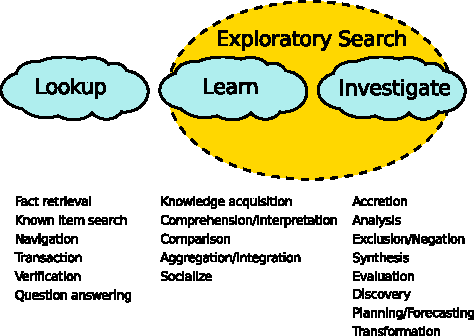
\includegraphics[bb=0 0 228 162]{clouds}
%\caption{Three clouds}
%\label{fig:clouds}
%\end{figure}

\section{User modeling in exploratory search}
Generally
\cite{oconnor10}, \cite{sugi04}, \cite{white07}, \cite{kules09}

\subsection{User Model Construction Methods}

\subsection{Utilizing the User Model}

Search interface and search results, how they are affected by User Model?

Stereotypes used? Personalization used?

\subsection{Experience}

How has user modeling been used in supporting exploratory search, example cases? What challenges have emerged? 

- Cases

\subsection{Analysis}

- Challenges
- Success
- Failures

\subsection{Recommendations, Future improvement needs etc.}

See Cases: Conclusions

\section{Conclusion}
Goal, solution summary

Our goal was to explore the field of Exploratory Search and User Modeling. We found several articles that have some contribution to the topic.

Summary of results and their reliability 

We found that:
- Usage
- Success
- Failures

How much is it used in the real world, really?

Research impact
- What has the research brought into software development?

\nocite{*} %tämä listaa kaikki viitteet luetteloon vaikka niitä ei olisi vielä viitattu

% Balancing columns in a ref list is a bit of a pain because you
% either use a hack like flushend or balance, or manually insert
% a column break.  http://www.tex.ac.uk/cgi-bin/texfaq2html?label=balance
% multicols doesn't work because we're already in two-column mode,
% and flushend isn't awesome, so I choose balance.  See this
% for more info: http://cs.brown.edu/system/software/latex/doc/balance.pdf
%
% Note that in a perfect world balance wants to be in the first
% column of the last page.
%
% If balance doesn't work for you, you can remove that and
% hard-code a column break into the bbl file right before you
% submit:
%
% http://stackoverflow.com/questions/2149854/how-to-manually-equalize-columns-
% in-an-ieee-paper-if-using-bibtex
%
% Or, just remove \balance and give up on balancing the last page.
%
\balance

% If you want to use smaller typesetting for the reference list,
% uncomment the following line:
% \small
\bibliographystyle{acm-sigchi}
\bibliography{umines}
\end{document}
